% Use only LaTeX2e, calling the article.cls class and 12-point type.

\documentclass[11pt]{article}
\usepackage[table]{xcolor}% http://ctan.org/pkg/xcolor
\usepackage{times}
\usepackage{graphicx}
\graphicspath{{figures/}} %Setting the graphicspath
\usepackage{caption}
\usepackage{subcaption}
\usepackage{enumitem}
\usepackage{multirow}

\usepackage[breakable]{tcolorbox}
\tcbset{nobeforeafter} % prevents tcolorboxes being placing in paragraphs

%\usepackage{breakurl}
%\usepackage{url}
%%% --- The following two lines are what needs to be added --- %%%
%\setcounter{biburllcpenalty}{7000}
%\setcounter{biburlucpenalty}{8000}

\usepackage{color}   %May be necessary if you want to color links

%\usepackage[hyphens]{url}
\usepackage{hyperref}
%\PassOptionsToPackage{hyphens}{url}\usepackage{hyperref}

\hypersetup{
	%hidelinks, % Remove visible links altogether
	%urlbordercolor = 1 1 1, % Make URL link border white
	breaklinks=true,
    colorlinks=true, %set true if you want colored links
    linktoc=all,     %set to all if you want both sections and subsections linked
    linkcolor=blue,  %choose some color if you want links to stand out
}   

\usepackage{setspace}

% The following parameters seem to provide a reasonable page setup.

\topmargin 0.0cm
\oddsidemargin 0.2cm
\textwidth 16cm 
\textheight 21cm %21cm
\footskip 1.0cm %1.0cm


\renewcommand\refname{References and Notes}

\newcounter{lastnote}
\newenvironment{scilastnote}{%
\setcounter{lastnote}{\value{enumiv}}%
\addtocounter{lastnote}{+1}%
\begin{list}%
{\arabic{lastnote}.}
{\setlength{\leftmargin}{.22in}}
{\setlength{\labelsep}{.5em}}}
{\end{list}}


\begin{document} 

% Double-space the manuscript.

% Include your paper's title here

\title{Sentiment Analysis of Movie Reviews using a Deep Learning Convolutional Neural Network}

\author
{Ahrim Han, Ph.D.\\
\\
}

% Include the date command, but leave its argument blank.

\date{July 23, 2019}



%%%%%%%%%%%%%%%%% END OF PREAMBLE %%%%%%%%%%%%%%%%

% Make the title.

\maketitle 
\newpage

\doublespacing
\tableofcontents
\singlespacing
\newpage

\baselineskip24pt

\section{Introduction}

\paragraph*{Problem Statment.}

Sentiment analysis (or opinion mining) is the task of identifying and classifying the sentiment expressed in a piece of text as being positive or negative. 
%
Given a bunch of text, sentiment analysis classifies peoples’ opinions, appraisals, attitudes, and emotions toward products, issues, and topics. 
%
The sentiment analysis has a wide range of applications in industry from forecasting market movements based on sentiment expressed in news and blogs, identifying customer satisfaction and dissatisfaction from their reviews and social media posts. It also forms the basis for other applications like recommender systems. 

In the past years of studies, a review text was converted to fixed-length vector using bag-of-words and these vectors were later used to train the classifier such as Naive Bayes or Support Vector Machine. The major problem of the bag-of-words are the 1) lack of consideration of semantic relationship between words 2) data sparsity and high dimensionality. Moreover, as there are tons of reviews and posts on the web, there is a strong need for the more accurate and automated sentiment analysis technique.

%In recent years, there has been a key breakthrough that has led to great performance of neural network models on a suite of challenging natural language processing problems. 
In recent years, there has been a remarkable performance improvement
to Natural Language Processing (NLP) problems
by applying deep learning neural networks.
%
Therefore, in this project, I will build deep learning models using various parameters to classify the positive and negative movie reviews using the high-edge deep learning techniques. I will compare models and observe the parameters affecting the performance in accuracy.

\paragraph*{Expected Beneficiaries.}

Automated and accurate sentiment analysis techniques can be used to detect fake reviews, news, or blogs and are becoming more and more important due to the huge impact on the business markets \cite{DeepLearning_amazon} \cite{fakespot}. We provide the potential beneficiaries of this work.

\begin{itemize}
\item 	
Businesses can find consumer opinions and emotions about their products and services.
\item
E-commerce companies, such as Amazon and Yelp, can identify fake reviews. 
%
There are cases when the results are not consistent from the actual looks and the sentiment analysis (automated analysis). 
For example, if majority reviews are positive, but the sentiment analysis determines that reviews should not be positive.
%
Then the administrators should inspect the reviews manually if those are fake or not.
%
Fake reviews are not only damaging both competing companies and customers, but they also lead to reduced trust in e-commerce companies and lower sales.
\item
Potential customers also can know the opinions and emotions of existing users.
%
Customers also can use the system based on the sentiment analysis \cite{fakespot} and check if the reviews are reliable and trustable before they make the decisions on buying products or services.
\end{itemize}

\paragraph*{Approach.}

We prepare the movie review text data for classification with deep learning methods. We obtain the large data set of the movie reviews \cite{Stanford_movie_review_paper} \cite{Stanford_movie_review_dataset}. 
%
We clean the documents of text reviews by removing punctuations, stopwords, stemming and removing non-frequent words to prevent a model from overfitting. In this pre-processing of documents, we use the more sophisticated methods in the \href{https://www.nltk.org/}{NLTK python package}. 

To build a deep learning Convolutional Neural Network (CNN) model, we basically use the sequential model of Keras. 

\begin{enumerate}
	\item First, the Embedding layer is located. There are two ways of setting the embedding layer: using the pre-trained word embedding or training new embedding from scratch. For a pre-trained word embedding, we use the GloVe (Global Vectors for Word Representation) embeddings \cite{glove}.

\item Second, a series of convolution 1D Neural Network and pooling layers are added according to typical CNN for text analysis. Then, after flattening layer, fully connected Dense layers are added. Since this is a binary classification problem, we use the Sigmoid function as an activation function for the final Dense layer. To prevent overfitting, we add Dropouts to deactivate neurons randomly, which forces the network to learn a more balanced representation. 

\item Finally, we will make the different deep learning models by adjusting the parameters and will find the best accurate model. We later will investigate the features affecting the accuracy.
\end{enumerate}

\paragraph*{Results}
In the paper \cite{Stanford_movie_review_paper}, the performance of machine learning models are in range of 67.42\% to 88.89\%. The model performed best in the cross validated Support Vector Machine (SVM) when concatenated with bag of words representation. In this project, we generate the preliminary results, and the best accuracy of our deep learning models based on CNN is 90.14\%. 

\section{Data Preprocessing}
\label{Data Preprocessing}

In this section, we perform cleaning documents.
More details of the process for cleaning documents can be found in
\href{https://github.com/ahrimhan/data-science-project/blob/master/project2/cleaning_document.ipynb}{this IPython notebook}. 

\subsection{Environment and Data}

\paragraph*{Environment.}
For this project, we used \textbf{my own Linux machine having AMD Ryzen 7 2700X, 16GB Memory, Geforce RTX 2070}.

In addition, \textbf{Keras with Tensorflow backend} is used for making a deep learning model.
%
Keras is a high-level API, written in Python and capable of running on top of TensorFlow, Theano, or CNTK deep learning frameworks. Keras provides a simple and modular API to create and train Neural Networks, hiding most of the complicated details under the hood. By default, Keras is configured to use Tensorflow as the backend since it is the most popular choice. Keras is becoming super popular recently because of its simplicity.


\paragraph*{Data.}
There is a large dataset for binary sentiment classification of movie reviews \cite{Stanford_movie_review_paper} \cite{Stanford_movie_review_dataset}. It contains substantially more data than previous benchmark datasets. 
This data set contains 50,000 reviews which is evenly split into two groups:
25,000 highly polar movie reviews for training and 25,000 for testing. 
\textbf{The train and test sets contain a disjoint set of movies}, so no significant performance is obtained by memorizing movie-unique terms and their associated with observed labels.  
Therefore, we can assume that the validation result with testing data set can be applicable for other movie reviews.

Each group has the same number of positive and negative reviews: a positive review has a score from 7 to 10 while a negative review has a score from 1 to 4. The reviews having score 5 or 6 are excluded to avoid vagueness.

For building deep learning models, all the documents are loaded as in Figure \ref{fig:data_loading}. The data sets for training and testing are stored in \texttt{data/train} and \texttt{data/test}, respectively. For each data set, positive and negative reviews are stored in \texttt{pos} and \texttt{neg} sub-directories.
%
I have attached the progress bars using the \href{https://github.com/tqdm/tqdm}{tqdm library}, which is useful in dealing with large data by allowing us to estimate each time of the stages.

%====================
\begin{figure}[h!]
\centering 
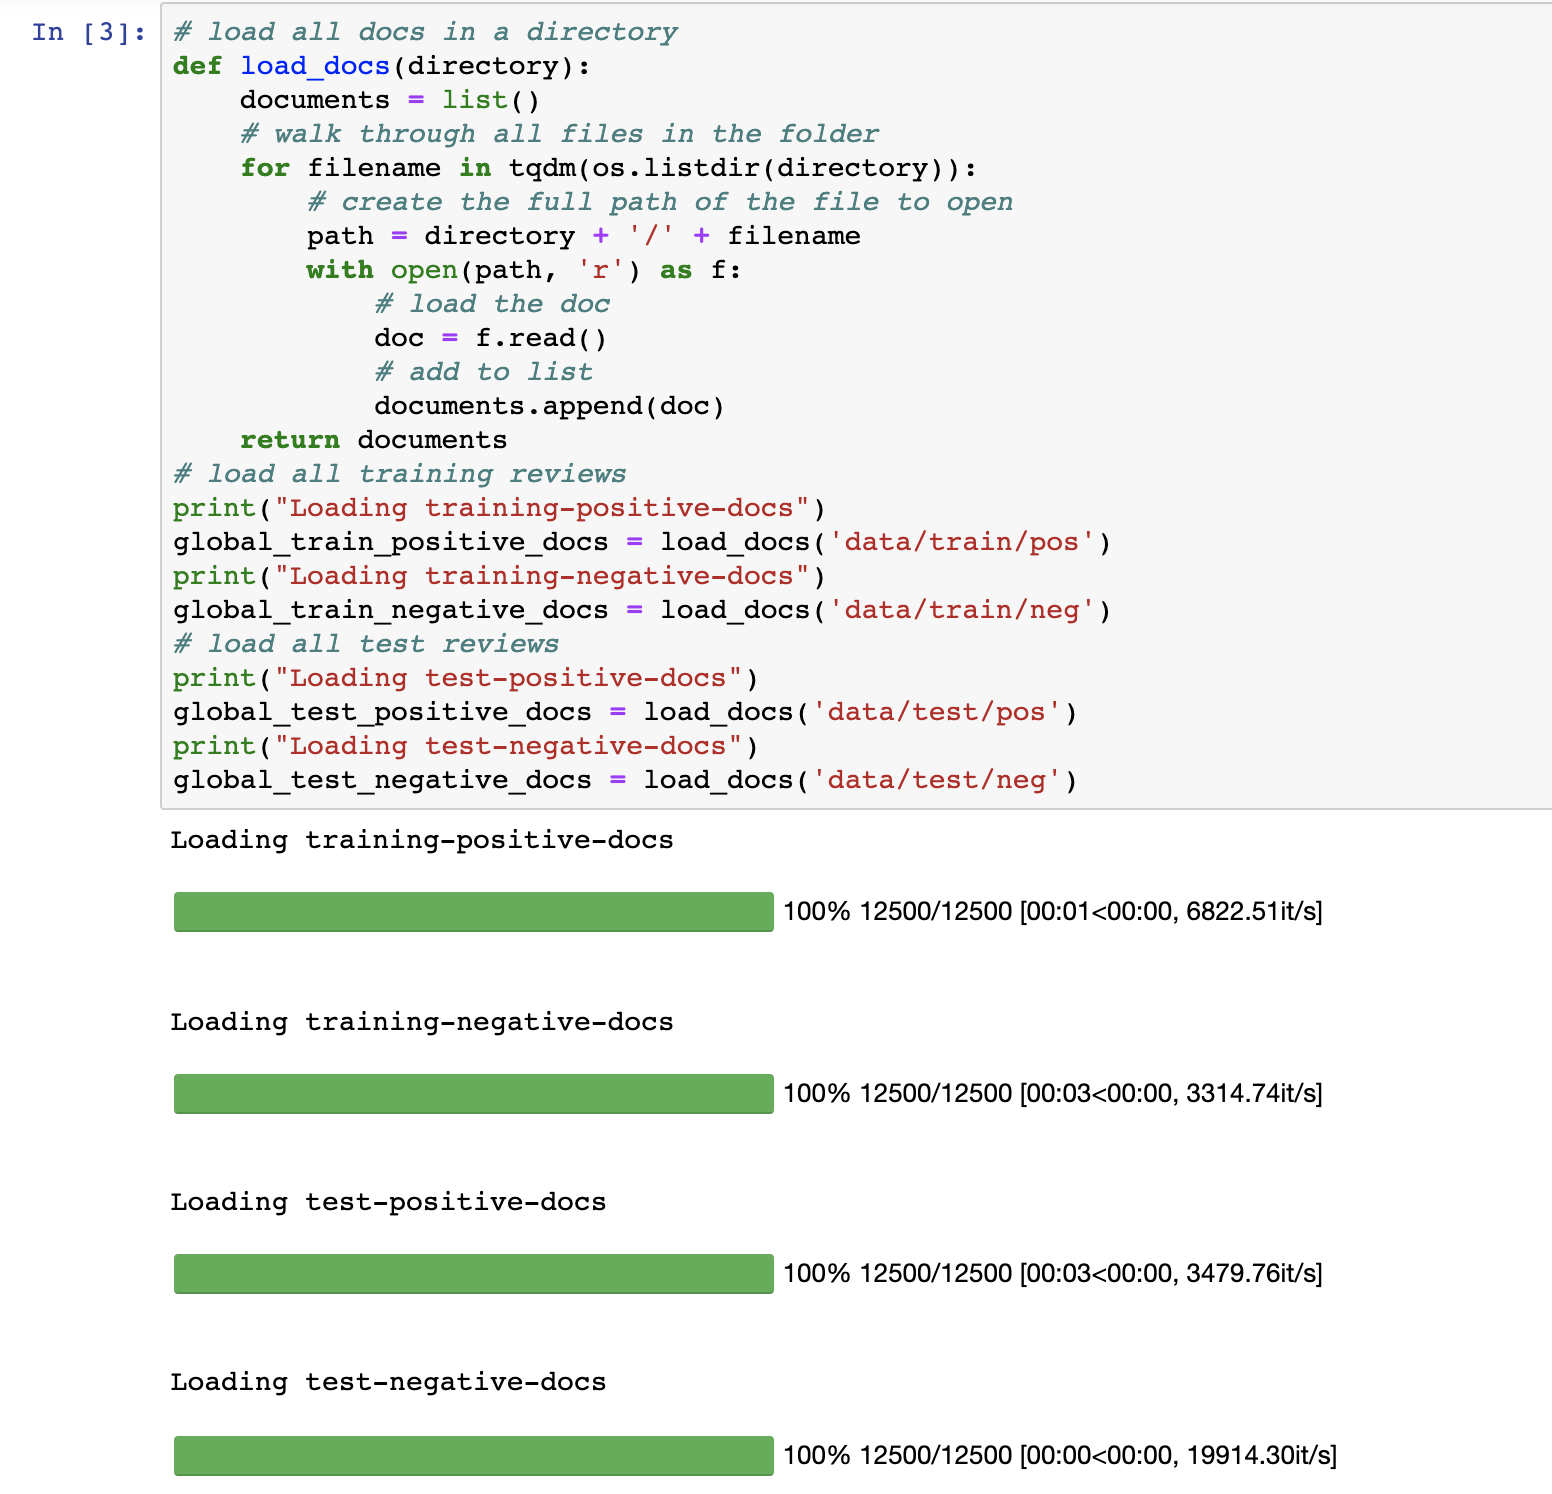
\includegraphics[width=\textwidth]{data_loading.png}
\caption{Data Loading.}
  \label{fig:data_loading}
\end{figure}
%====================

\subsection{Cleaning Documents}

In most of NLP releated works, documents are normally pre-processed to get better performance.
We tried to apply several techniques which are well-known as follows:

\begin{enumerate}
	\item \textbf{Removing punctuations.} 
Normally punctuations do not have any meaning, but they exist for understandability. Therefore, such punctuations should be removed. But, we did not remove the apostrophe mark (') since such removing caused the incorrect stemming.

\item \textbf{Removing stopwords.}
We filtered out the stopwords.
The stop words are those words that do not contribute to the deeper meaning of the phrase.
They are the most common words such as: ``the", ``a", and ``is".
\texttt{NLTK} python package provides a list of commonly agreed upon stop words for a variety of languages.

\item \textbf{Stemming.}  
The \texttt{PorterStemmer} is provided in \texttt{NLTK} python package.
We made the words into lowercases and used the stemming method in order to both reduce the vocabulary and to focus on the sense or sentiment of a document rather than deeper meaning.

\item \textbf{Defining a vocabulary dictionary of preferred words and removing non-frequent words.}   
It is important to define a vocabulary of known words when using a bag-of-words or embedding model.
The more words, the larger the representation of documents, therefore it is important to constrain the words to only those believed to be predictive. 

In this project, \textbf{we set up the vocabulary dictionary and remove the non-frequent words to prevent a model from overfitting.} 
Building code of the vocabulary dictionary is implemented in \href{https://github.com/ahrimhan/data-science-project/blob/master/project2/vocab.ipynb}{\texttt{vocab.ipynb} notebook}. 
The process can be summarized as follows.

\begin{itemize}
\item First, based on only reviews in the training dataset, we count the words' occurrences using \texttt{Counter} function. This is saved in 
\href{https://github.com/ahrimhan/data-science-project/tree/master/project2/vocab/vocab
_counter.txt}{\texttt{vocab\_counter.txt}} file and contains 52,826 words.
%
Figure \ref{fig:most_frequent_words} shows the most frequent 30 words extracted from training data set.
%====================
\begin{figure}[h!]
\centering 
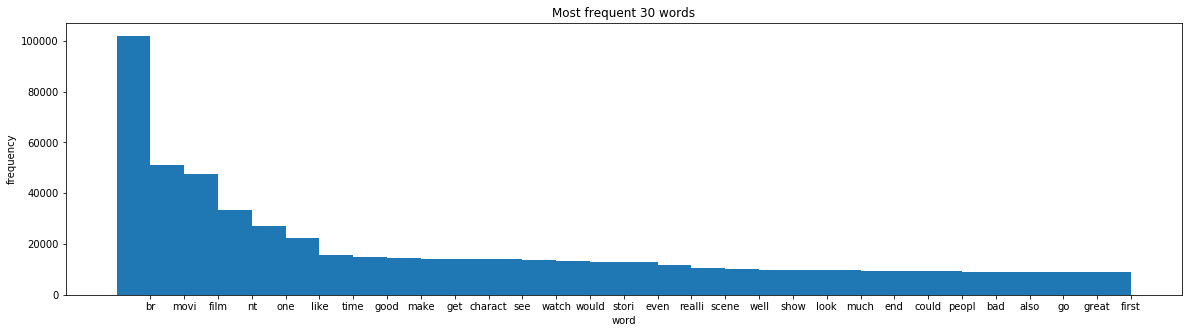
\includegraphics[width=\textwidth]{most_frequent_words.png}
\caption{Most Frequent 30 Words in Training Data Set.}
  \label{fig:most_frequent_words}
\end{figure}
%====================

\item Then, we filter out the words that have low occurrences, such as only being used once or none and set up the vocabulary dictionary. Thus, the vocabularies have the two or more occurrences. There are 30,819 number of words in the vocabulary dictionary and those are saved in the \href{https://github.com/ahrimhan/data-science-project/tree/master/project2/vocab/vocab.txt}{\texttt{vocab.txt}} file.

\item
Finally, using the vocabulary dictionary, we remove the non-frequent words for cleaning documents. This is done by filtering out words that are not in the vocabulary dictionary and removing all words that have a length $<=$ 1 character.
\end{itemize}

\end{enumerate}

\subsection{Multiprocessing}
Pre-processing mentioned above requires heavy computation. 
To improve the speed, we parallelized the pre-processing using the \textbf{Pool module} in \textbf{multiprocessing package}.
Since we use a CPU having 8 cores, the size of Pool is set as 8.
By using this technique, \textbf{we could achieve 6 to 7 times speed up.} 
Using the single thread, it takes 10 to 12 minutes for cleaning up 12,500 documents, whereas, using the multiple threads, it takes only 1 minute and 20 to 40 seconds.

\subsection{Data Encoding}


To use documents as an input of a model, each document is encoded as a sequence object of Keras.

First, we encode the documents as sequence objects.
We pad all reviews to the length of the longest review in the training dataset.
We can find the longest review using the \texttt{max()} function on the training dataset and take its length. 
We can then call the Keras function \texttt{pad\_sequences()} to pad the sequences to the maximum length by adding 0 values on the end.

We create a list of labels: `0' for negative reviews and `1' for positive reviews.
We do not need the one-hot-encoding process (a function called \texttt{to\_categorical()} in Keras) because there is only two classes of positive and negative.

\section{Building Deep Learning Models}
\label{Building Deep Learning Models}

To build a deep learning model, we basically use the sequential model of Keras.
%
The model is built in the following steps as in Figure \ref{fig:building_model}.
\begin{enumerate}
	\item First, the Embedding layer is located. There are two options of setting embedding layers: using the pre-trained word embedding or training new embedding from scratch.
\item Second, a series of \textbf{convolution 1D} and \textbf{pooling layers} are added according to typical CNN for text analysis. 
%
In order to check the effects of the number of convolution layers, we made the function below configurable to set the number of additional convolution layers.
\item Then, after flattening layer, fully connected Dense layers are added.
Since this is a binary classification problem to output a value between 0 and 1 for the negative and positive sentiment in the review, we use the Sigmoid function as an activation function for the final output Dense layer. 
%
If you try to predict a score of a review, it would be better to use 'softmax' function as the activation function.
%classification, which are flatten and fully connected layers.

\end{enumerate}

%====================
\begin{figure}[h!]
\centering 
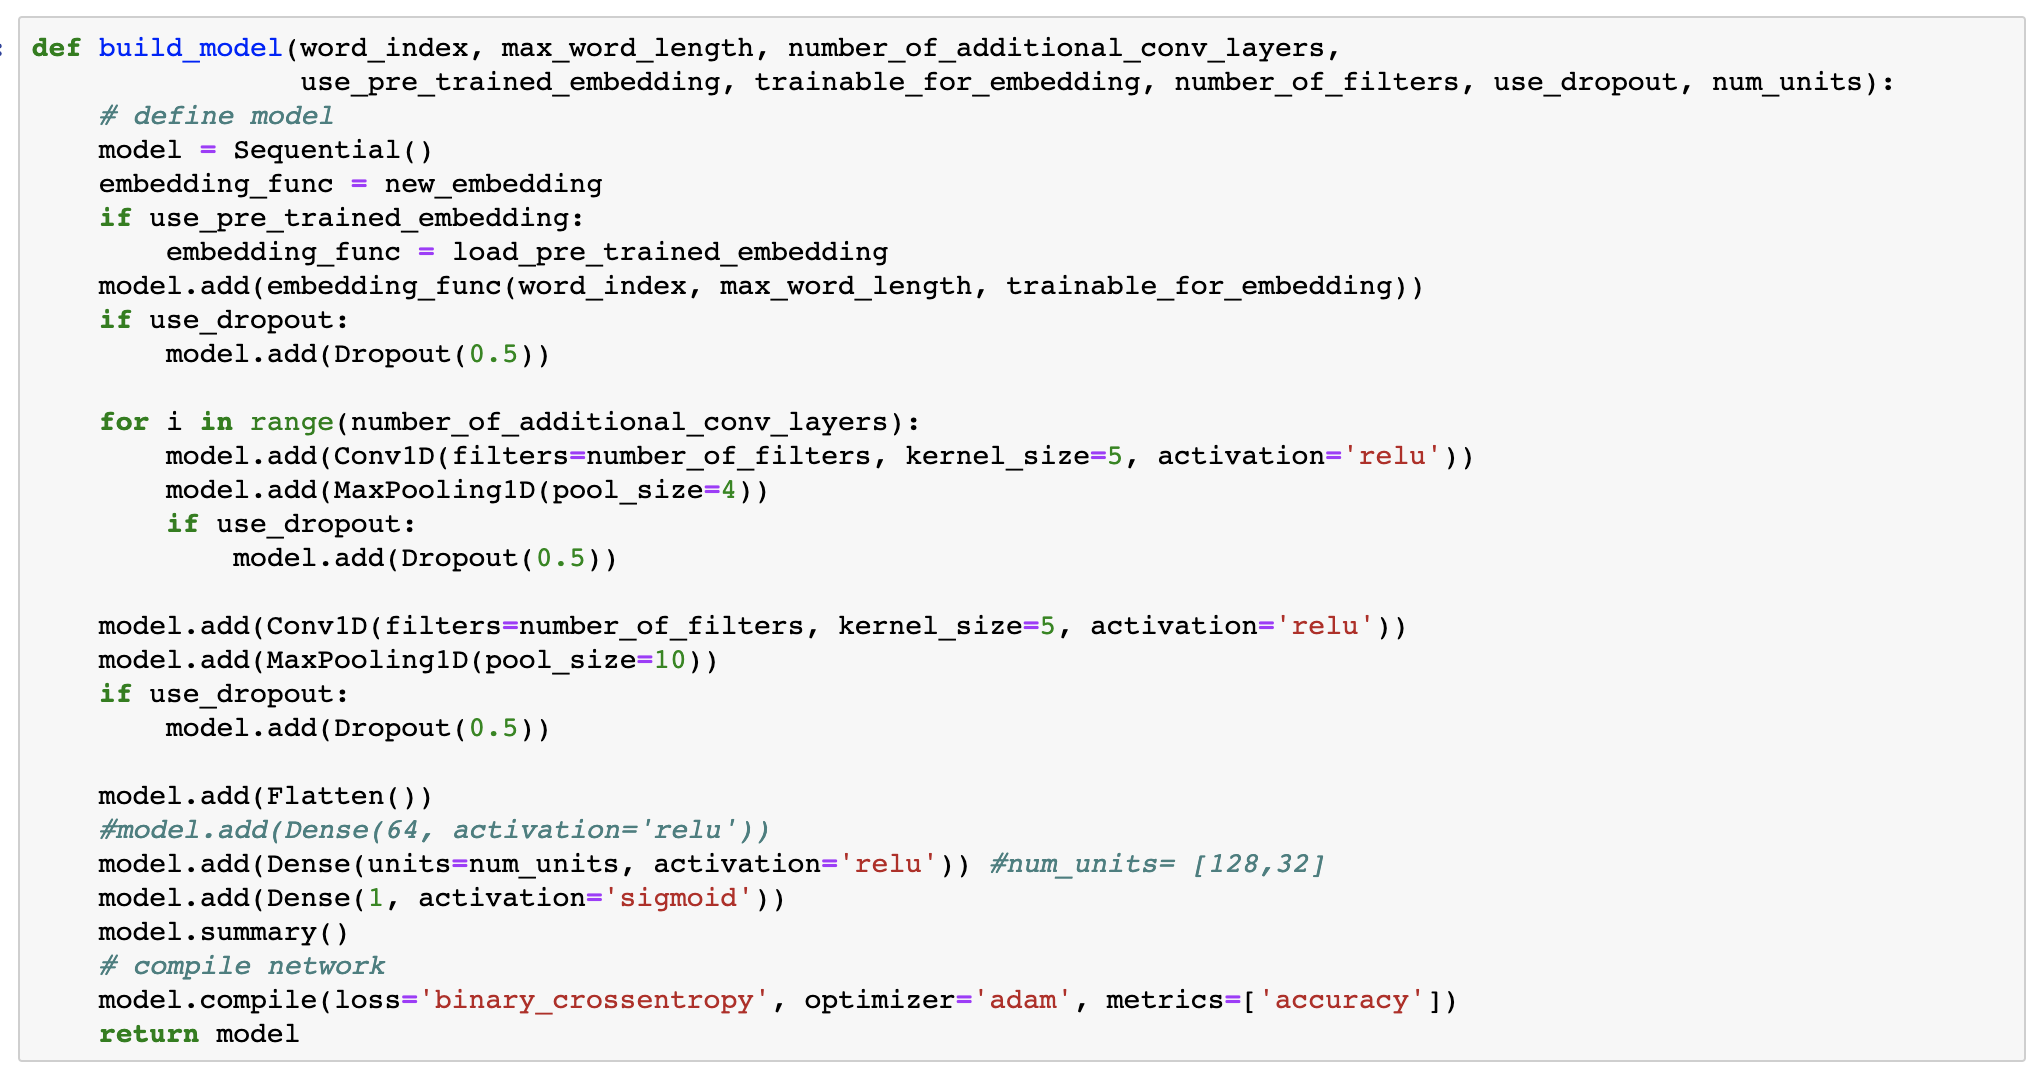
\includegraphics[width=\textwidth]{building_model.png}
\caption{Building a Deep Learning Model.}
  \label{fig:building_model}
\end{figure}
%====================


\subsection{Embedding Layers with Word Embeddings}

A word embedding is a way of representing text where each word in the vocabulary is represented by a real valued vector in a high-dimensional space. The vectors are learned in such a way that words that have similar meanings will have similar representation in the vector space (close in the vector space). This is a more expressive representation for text than more classical methods like bag-of-words, where relationships between words or tokens are ignored, or forced in bigram and trigram approaches.

We have two options for using word embeddings on natural language processing projects: \textbf{learning an embedding or reusing an embedding.}
%
If choosing to learn own embedding, this requires a large amount of text data to ensure that useful embeddings are learned. Therefore, \textbf{it is common to use pre-trained word embeddings, such as Word2Vec and Glove} available for free download.
%
These can be used instead of training from scratch.

Learning a word embedding while training a neural network is a common technique to deal with texts in Deep Learning.
%
To investigate the effectiveness of the existence of pre-trained word embedding,
each of the 1) pre-trained word embedding and the 2) new (not-trained) embedding, and the
3) updated pre-trained embedding (i.e., pre-trained embedding is used to seed the model, but the embedding is updated jointly during the training of the model) are used for building models and the accuracy of those models are compared.

Keras offers an Embedding layer that can be used for neural networks on text data.
%
It requires that the input data be integer encoded, so that each word is represented by a unique integer. This data preparation step can be performed using the Tokenizer API also provided with Keras.
%
This is well explained in \href{https://blog.keras.io/using-pre-trained-word-embeddings-in-a-keras-model.html}{this blog}.

\subsubsection{Pre-Trained Word Embedding: Glove}

In this project, we use the \href{https://nlp.stanford.edu/projects/glove/}{GloVe}. GloVe stands for ``Global Vectors for Word Representation" and is an unsupervised learning algorithm for obtaining vector representations for words.
It is a somewhat popular embedding technique based on factorizing a matrix of word co-occurence statistics.
%
Specifically, we use the 200-dimensional GloVe embeddings of 400k words computed on a 2014 dump of English Wikipedia. You can download these data \href{http://nlp.stanford.edu/data/glove.6B.zip}{here}.
%
In addition, to check whether the pre-trained word embedding needs to be trained or not, we made the function below configurable for the \textit{trainable} parameter of Embedding object.

\subsubsection{Training New Word Embedding}

We can perform by not using pre-trained word embeddings, but instead initializing our Embedding layer from scratch and learning its weights during training. 
%
\textbf{New word embedding is created with no pre-trained weights}, so the \textit{trainable} parameter should always be ``True".
Figure \ref{fig:word_embedding_code} shows the python code to return the Embedding layer that is used 
to load a pre-trained word embedding or 
to learn a new word embedding.
 
%====================
\begin{figure}[h!]
\centering 
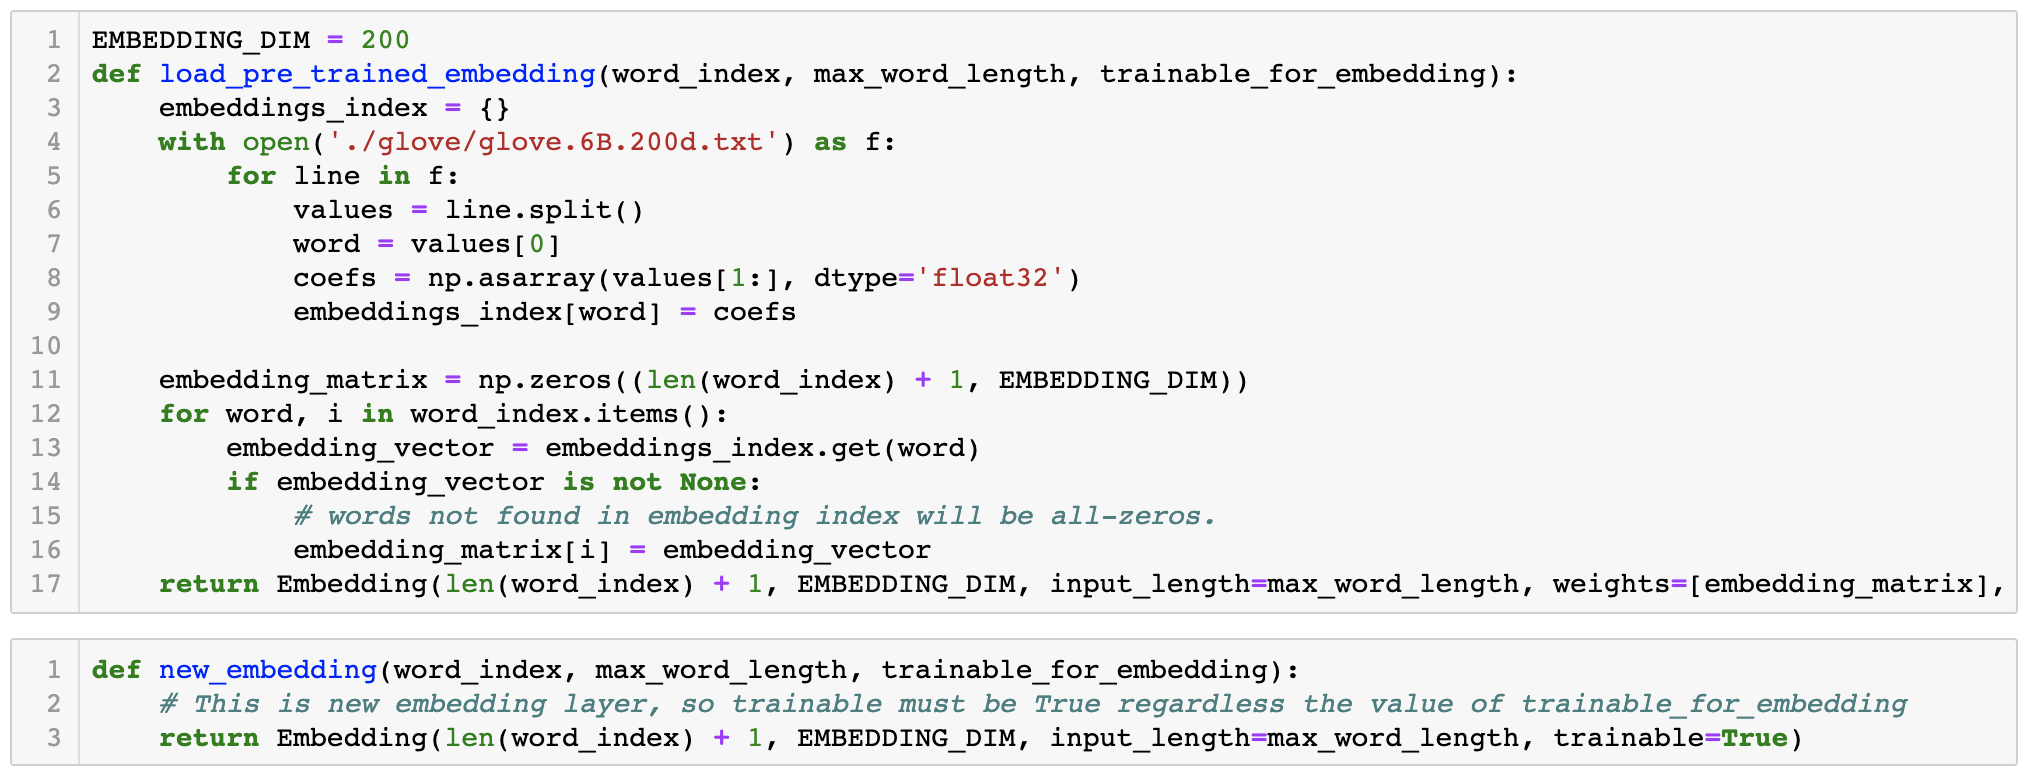
\includegraphics[width=\textwidth]{word_embedding_code.png}
\caption{Embedding Layers with Word Embeddings.}
  \label{fig:word_embedding_code}
\end{figure}
%====================

%We can now add this Embedding layer to our model. We also have a slightly different model configuration with a lot more filters (128) in the CNN model and a kernel that matches the 5 words used as neighbors when developing the word2vec embedding. Finally, the back-end of the model was simplified.

\subsection{1-Dimensional Convolutional Neural Network (CNN) and Pooling}

We use a CNN as they have proven to be successful at document classification problems.
A conservative CNN configuration is used with 32 filters (parallel fields for processing words) and a kernel size of 8.
We used the 96 filters and 5 kernels by default
with a rectified linear (`ReLU') activation function.
%
We will adjust the number of filters to investigate if they affect the accuracy of models.
%
This extracted set of features are then passed to MaxPooling layer, which filters the dominating terms from the extracted features.

\subsection{Activation functions and Dropout}

\paragraph*{Activation Function.}  
  The activation function is used as a decision making body at the output of a neuron. The neuron learns Linear or Non-linear decision boundaries based on the activation function.
%
It also has a normalizing effect on the neuron output which prevents the output of neurons after several layers to become very large, due to the cascading effect.  

%
There are three most widely used activation functions. We used ReLU and Sigmoid.
\begin{itemize}
\item \textbf{Sigmoid}: It maps the input (x axis) to values between 0 and 1 (which may later results in the \href{https://towardsdatascience.com/the-vanishing-gradient-problem-69bf08b15484}{vanishing gradient problem}).
\item \textbf{Tanh}: It is similar to the Sigmoid function but maps the input to values between -1 and 1.
\item \textbf{Rectified Linear Unit (ReLU)}: - It allows only positive values to pass through it. The negative values are mapped to zero.
\end{itemize}

\paragraph*{Dropout.}
 During training, when dropout is applied to a layer, some percentage of its neurons (a hyperparameter, with common values being between 20\% and 50\%) are randomly deactivated or ``dropped out" along with their connections. Which neurons are dropped out are constantly shuffled randomly during training. This forces the network to learn a more balanced representation, and \textbf{dropouts are known to help prevent overfitting}.

\section{Training Deep Learning Models}
\label{Training Deep Learning Models}

\subsection{Model Configurations}

All the functions defined above are integrated into the \texttt{build\_and\_train\_model} function.
Each model is trained by different combinations of six parameters, and
we compare the accuracy of those models.

%
The meanings of parameters can be explained as follows:
\begin{enumerate}
\item \textbf{use\_cleaned\_docs}: Cleaning review documents or not. 
\item \textbf{number\_of\_additional\_conv\_layers}: Number of additional convolution layers (0,2). Basically, one convolution layer is used (`number\_of\_additional\_conv\_layers'=0). If you want to add more convolution layers, we can adjust this parameter to a higher number. For experiment, we adjust the `number\_of\_additional\_conv\_layers'=2, so the total convolution layers becomes 3.
\item \textbf{use\_pre\_trained\_embedding}: Using pre-trained embedding or not. If True, the GloVe embedding will be used as mentioned above.
\item \textbf{trainable\_for\_embedding}: Training the embedding layer with training data set or freezing. Note, when using the new embedding layer, then `trainable\_for\_embedding' should be True.
\item \textbf{number\_of\_filters}: Number of filters in the convolution layers (96, 48, and 24).
%conventional : 32 filters with 8 kernel for multiprocessors
\item \textbf{use\_dropout}: Using Dropout or not. In the experiment, 50\% percentage of its neurons are randomly deactivated.
\item \textbf{num\_units}: Number of units in Dense layer. This reduces the capacity of network (128, 64, 32, 8). 
\end{enumerate}

When setting up model configurations by combination of features, there are no cases of no embedding layers 
(`use\_pre\_trained\_embedding'= False and `trainable\_for\_embedding' = False), so these should be eliminated.

\textbf{We use the callbacks functions of \texttt{EarlyStoppig} and \texttt{ModelCheckpoint}.}
%
One way to avoid overfitting is to terminate the process early.
We used the \textbf{\texttt{EarlyStoppig} function and set the arguments `monitor'= val\_acc (test accuracy) and `patience'=2.}
The `patience' indicates the number of epochs with no improvement after which training will be stopped.
%
The \texttt{ModelCheckpoint} callback saves the model after every epoch. 

\subsection{Results of Models}

Table \ref{table:acc_classification} shows the accuracy of classification results for the deep learning CNN models and configurations.
%best accuracy
\noindent In those models, the Model 11 has the best accuracy of 90.14\% (highlighted in red), and the Model 5 has the second best accuracy of 89.73\% (highlighted in green). 

%====================
\begin{table}[h!]
\centering
\begin{tabular}{||c|c|c|c|c|c|c|c|c||}
\hline
Model \# & clean\_docs &	\# conv.	& pre-trained &	trainable &	\# filters	& dropout &	\# units & Accuracy\\
\hline
Model 0   & FALSE	 & 0	&TRUE	&FALSE	&96	&FALSE	&128 & 86.62\\
\hline
Model 1	&	FALSE	&	0	&	FALSE	&	TRUE	&	96	&	FALSE	&	128	&	87.50\\
\hline
Model 2	&	FALSE	&	0	&	TRUE	&	TRUE	&	96	&	FALSE	&	128	&	88.82\\
\hline
Model 3	&	FALSE	&	2	&	TRUE	&	FALSE	&	96	&	FALSE	&	128	&	88.63\\
\hline
Model 4	&	FALSE	&	2	&	FALSE	&	TRUE	&	96	&	FALSE	&	128	&	89.11\\
\hline
\cellcolor{green!25}Model 5	&	\cellcolor{green!25}FALSE	&	\cellcolor{green!25}2	&	\cellcolor{green!25}TRUE	&	\cellcolor{green!25}TRUE	&	\cellcolor{green!25}96	&	\cellcolor{green!25}FALSE	&	\cellcolor{green!25}128	&	\cellcolor{green!25}89.73\\
\hline
Model	6	&	FALSE	&	0	&	TRUE	&	TRUE	&	24	&	FALSE	&	32	&	88.39	\\
\hline
Model	7	&	FALSE	&	0	&	TRUE	&	TRUE	&	24	&	TRUE	&	32	&	89.49	\\
\hline
Model	8	&	FALSE	&	2	&	TRUE	&	TRUE	&	48	&	FALSE	&	128	&	89.62	\\
\hline
Model	9	&	FALSE	&	2	&	TRUE	&	TRUE	&	24	&	FALSE	&	128	&	89.51	\\
\hline
Model	10	&	FALSE	&	2	&	TRUE	&	TRUE	&	96	&	FALSE	&	32	&	89.42	\\
\hline
\cellcolor{red!25}Model	11	&	\cellcolor{red!25}FALSE	&	\cellcolor{red!25}2	&	\cellcolor{red!25}TRUE	&	\cellcolor{red!25}\cellcolor{red!25}TRUE	&	\cellcolor{red!25}96	&	\cellcolor{red!25}FALSE	&	\cellcolor{red!25}64	&	\cellcolor{red!25}90.14	\\
\hline
Model	12	&	FALSE	&	2	&	TRUE	&	TRUE	&	96	&	FALSE	&	8	&	89.20	\\
\hline
Model	13	&	FALSE	&	2	&	TRUE	&	TRUE	&	24	&	FALSE	&	32	&	89.12	\\
\hline
Model	14	&	FALSE	&	2	&	TRUE	&	TRUE	&	96	&	TRUE	&	128	&	89.18	\\
\hline
Model	15	&	FALSE	&	2	&	TRUE	&	TRUE	&	48	&	TRUE	&	128	&	88.99	\\
\hline
Model	16	&	TRUE	&	2	&	TRUE	&	TRUE	&	96	&	TRUE	&	128	&	86.98	\\
\hline
Model	17	&	TRUE	&	2	&	TRUE	&	TRUE	&	96	&	FALSE	&	128	&	87.36	\\
\hline
\end{tabular}
\caption{Results of the accuracy of classification for the deep learning models and configurations.}
\label{table:acc_classification}
\end{table}
%====================

\noindent The abbreviated terms in Table \ref{table:acc_classification} are as follows:
\begin{itemize}
\setlength\itemsep{-1em}
\item use\_cleaned\_docs: clean\_docs
\item number\_of\_additional\_conv\_layers: \# conv.
\item use\_pre\_trained\_embedding: pre-trained
\item trainable\_for\_embedding: trainable
\item number\_of\_filters: \# filters
\item use\_dropout: dropout
\item num\_units: \# units
\end{itemize}


Figure \ref{fig:model11config} represents the model configuration and training progress of Model 11.
%====================
\begin{figure}[h!]
\centering 
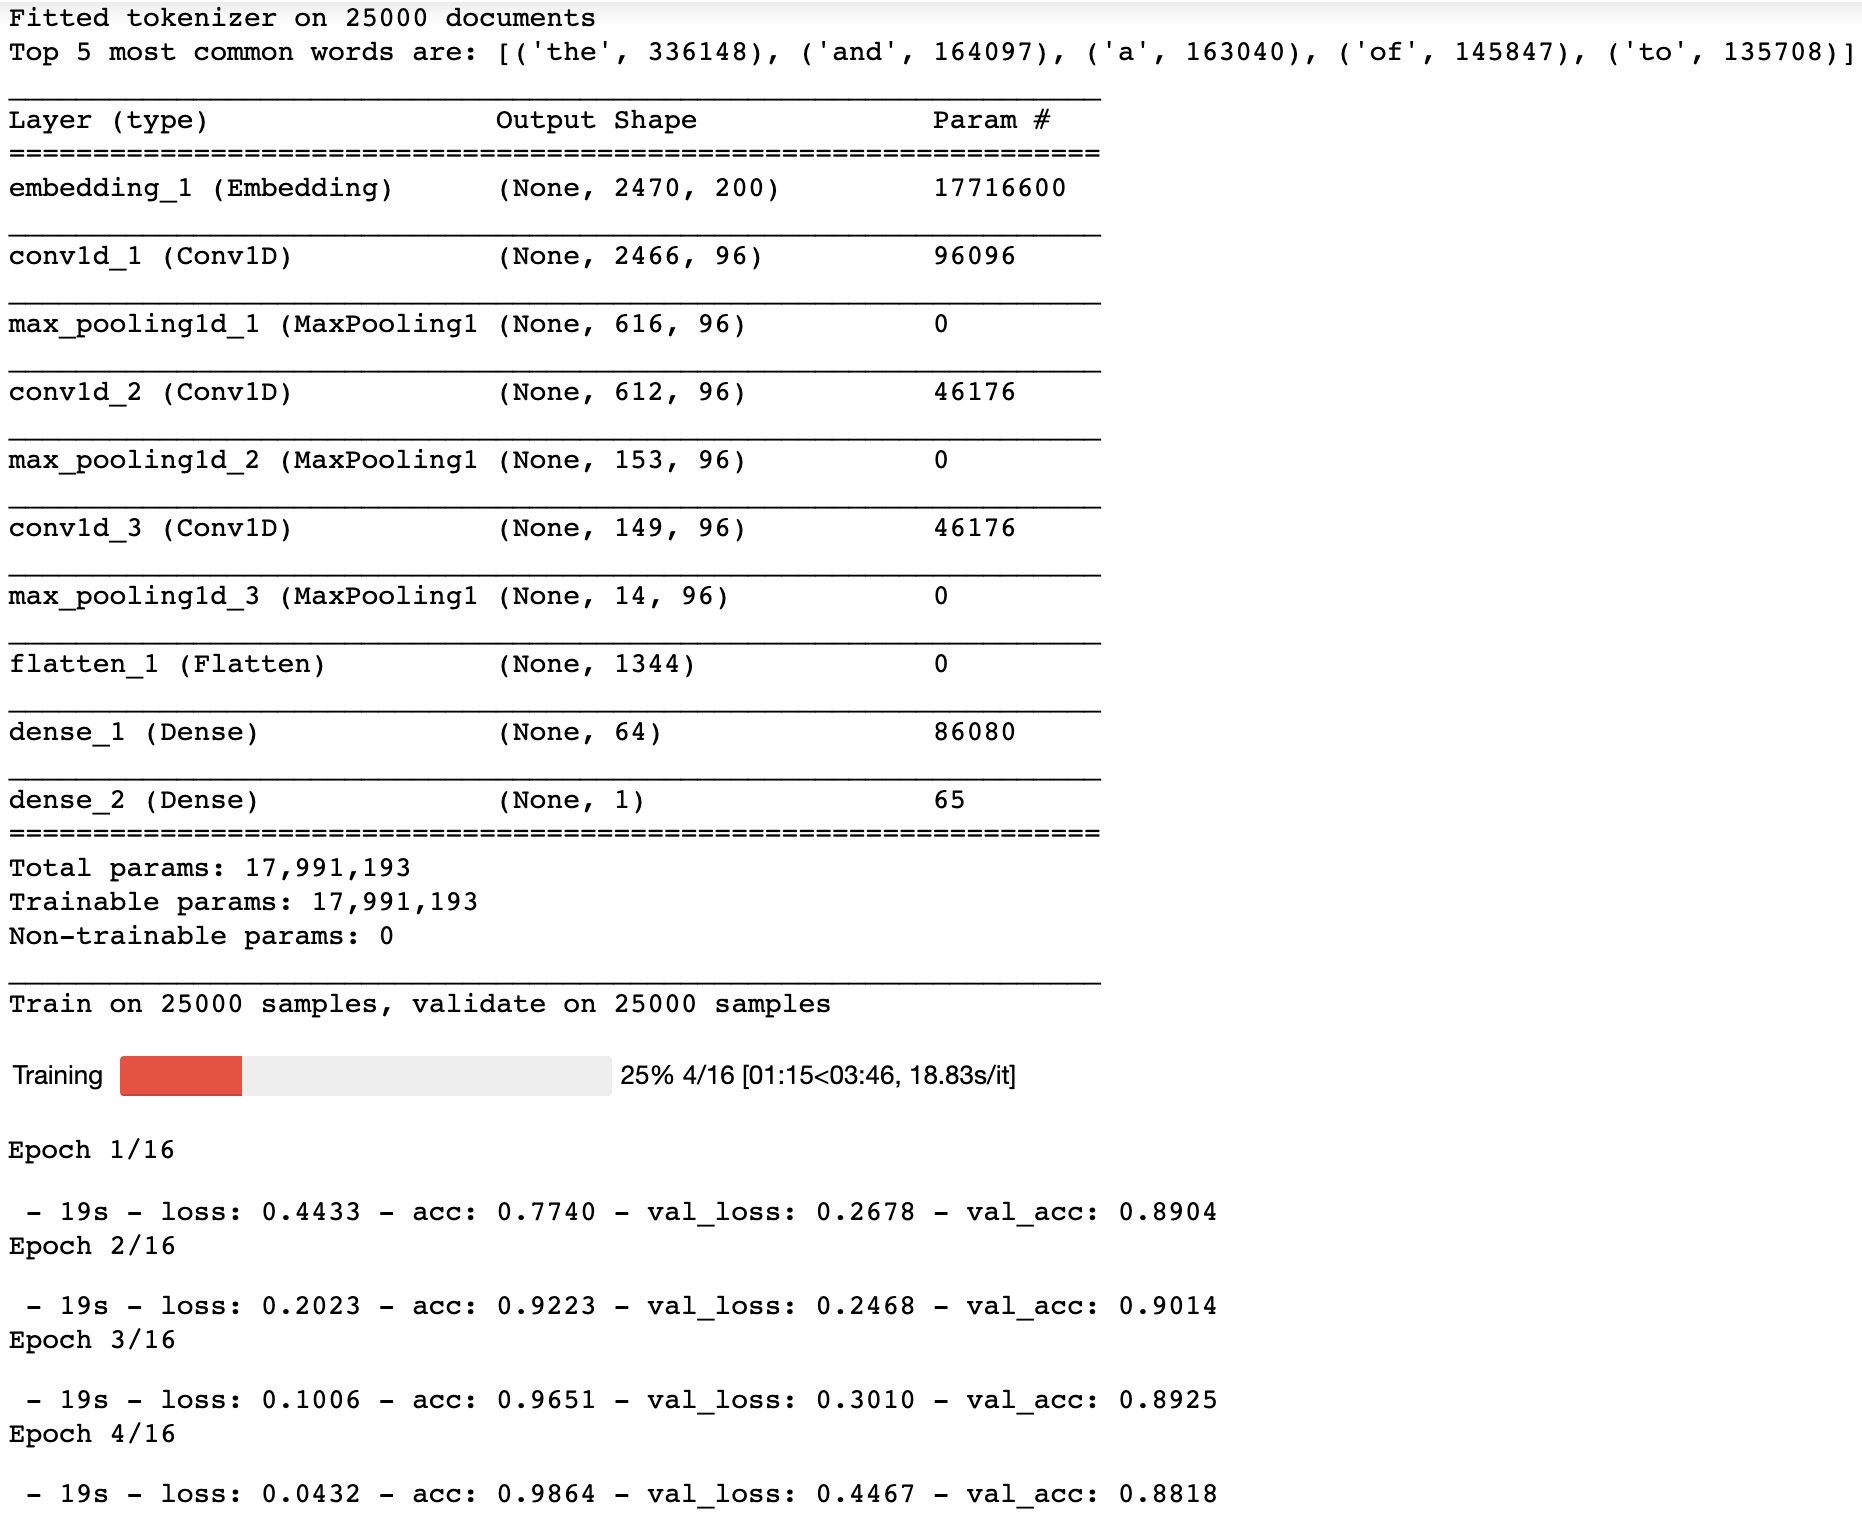
\includegraphics[width=\textwidth]{model11_config.png}
\caption{Model 11: model configuration and training progress.}
  \label{fig:model11config}
\end{figure}
%====================

\subsubsection{Effect of the Use of Word Embeddings}

For the word embedding, the \textbf{use of sole pre-trained word embedding produces the least performance.} This can be interpreted that Embedding model cannot be generalized and should be trained into their contexts. Rather, the \textbf{use of the new training word embedding was the better choice.}

As highlighted in Table \ref{table:acc_wordembedding}, most of all, \textbf{models that use the pre-trained word embedding and updating weights during training provide the best performance.}.
Using the pre-trained word embedding produces the better performance takes advantages of leveraging massive datasets with a vast corpus of language capturing word meanings in a statistically robust manner. It is difficult to train from scratch, therefore, we need to use the pre-defined word embedding and customize it into our dataset at the same time.

%====================
\begin{table}[h!]
\centering
\begin{tabular}{||c|c|c|c|c|c|c|c|c||}
\hline
Model \# & clean\_docs &	\# conv.	& pre-trained &	trainable &	\# filters	& dropout &	\# units & Accuracy\\
\hline
Model 0   & FALSE	 & 0	&\cellcolor{yellow!25}TRUE	&\cellcolor{yellow!25}FALSE	&96	&FALSE	&128 & 86.62\\
\hline
Model 1	&	FALSE	&	0	&	\cellcolor{yellow!25}FALSE	&	\cellcolor{yellow!25}TRUE	&	96	&	FALSE	&	128	&	87.50\\
\hline
Model 2	&	FALSE	&	0	&	\cellcolor{blue!25}TRUE	&	\cellcolor{blue!25}TRUE	&	96	&	FALSE	&	128	&	\cellcolor{blue!25}88.82\\
\hline
\hline
Model 3	&	FALSE	&	2	&	\cellcolor{yellow!25}TRUE	&	\cellcolor{yellow!25}FALSE	&	96	&	FALSE	&	128	&	88.63\\
\hline
Model 4	&	FALSE	&	2	&	\cellcolor{yellow!25}FALSE	&	\cellcolor{yellow!25}TRUE	&	96	&	FALSE	&	128	&	89.11\\
\hline
Model 5	&	FALSE	&	2	&	\cellcolor{blue!25}TRUE	&	\cellcolor{blue!25}TRUE	&	96	&	FALSE	&	128	&	\cellcolor{blue!25}89.73\\
\hline
\end{tabular}
\caption{Accuracy results comparing of the use of word embeddings.}
\label{table:acc_wordembedding}
\end{table}
%====================

\subsubsection{Effect of the Number of Convolutional Network Layers and Filters}


\paragraph*{Number of CNN.} 
As highlighted in Table \ref{table:acc_numCNN}, the model with the additional 2 layers works better than the model with only one layer, but the difference is marginal. 
%====================
\begin{table}[h]
\centering
\begin{tabular}{||c|c|c|c|c|c|c|c|c||}
\hline
Model \# & clean\_docs &	\# conv.	& pre-trained &	trainable &	\# filters	& dropout &	\# units & Accuracy\\
\hline
Model	6	&	FALSE	&	\cellcolor{yellow!25}0	&	TRUE	&	TRUE	&	24	&	FALSE	&	32	&	88.39	\\
\hline
Model	13	&	FALSE	&	\cellcolor{blue!25}2	&	TRUE	&	TRUE	&	24	&	FALSE	&	32	&	\cellcolor{blue!25}89.12	\\
\hline
\hline
Model 2	&	FALSE	&	\cellcolor{yellow!25}0	&	TRUE	&	TRUE	&	96	&	FALSE	&	128	&	88.82\\
\hline
Model 5	&	FALSE	&	\cellcolor{blue!25}2	&	TRUE	&	TRUE	&	96	&	FALSE	&	128	&	\cellcolor{blue!25}89.73\\
\hline
\hline
Model 0   & FALSE	 & \cellcolor{yellow!25}0	&TRUE	&FALSE	&96	&FALSE	&128 & 86.62\\
\hline
Model 3	&	FALSE	&	\cellcolor{blue!25}2	&	TRUE	&	FALSE	&	96	&	FALSE	&	128	&	\cellcolor{blue!25}88.63\\
\hline
\hline
Model 1	&	FALSE	&	\cellcolor{yellow!25}0	&	FALSE	&	TRUE	&	96	&	FALSE	&	128	&	87.50\\
\hline
Model 4	&	FALSE	&	\cellcolor{blue!25}2	&	FALSE	&	TRUE	&	96	&	FALSE	&	128	&	\cellcolor{blue!25}89.11\\
\hline
\end{tabular}
\caption{Number of CNN layers (0,2): Results of the accuracy.}
\label{table:acc_numCNN}
\end{table}
%====================


\paragraph*{Number of Filters in CNN.}
Model 5, 8 and 9 represent the results of accuracy for the different number of filters 98, 48, and 24.
%
As highlighted in Table \ref{table:acc_numfiltersCNN}, 
the largest number of filters of 96 in convolutional neural network gives best performance (accuracy of 89.73\%). But it does not guarantee that the larger number of filters always produces the better performance.
%====================
\begin{table}[h]
\centering
\begin{tabular}{||c|c|c|c|c|c|c|c|c||}
\hline
Model \# & clean\_docs &	\# conv.	& pre-trained &	trainable &	\# filters	& dropout &	\# units & Accuracy\\
\hline
Model 5	&	FALSE	&	2	&	TRUE	&	TRUE	&	\cellcolor{blue!25}96	&	FALSE	&	128	&	\cellcolor{blue!25}89.73\\
\hline
Model	8	&	FALSE	&	2	&	TRUE	&	TRUE	&	\cellcolor{yellow!25}48	&	FALSE	&	128	&	89.62	\\
\hline
Model	9	&	FALSE	&	2	&	TRUE	&	TRUE	&	\cellcolor{yellow!25}24	&	FALSE	&	128	&	89.51	\\
\hline
\end{tabular}
\caption{Number of filters (98, 48, 24) in CNN: Results of the accuracy.}
\label{table:acc_numfiltersCNN}
\end{table}
%====================


\subsubsection{Effect of the Number of Units in Dense Layer}

As highlighted in Table \ref{table:acc_numUnitsDense}, the model with the 64 number of units in the Dense layer (Model 11) has the highest accuracy. Exception of that model, the larger number of units in the Dense layer has, the better performance.
%
In short, models have the higher accuracy in the order of the number of units of 128 (Model 5), 32 (Model 10), and 8 (Model 12).
%====================
\begin{table}[h]
\centering
\begin{tabular}{||c|c|c|c|c|c|c|c|c||}
\hline
Model \# & clean\_docs &	\# conv.	& pre-trained &	trainable &	\# filters	& dropout &	\# units & Accuracy\\
\hline
Model 5	&	FALSE	& 2	&	TRUE	&	TRUE	&	96	&	FALSE	&	\cellcolor{yellow!25}128	&	89.73\\
\hline
Model	10	&	FALSE	&	2	&	TRUE	&	TRUE	&	96	&	FALSE	&	\cellcolor{yellow!25}32	&	89.42	\\
\hline
Model	11	&	FALSE	&	2	&	TRUE	&	TRUE	&	96	&	FALSE	&	\cellcolor{blue!25}64	&	\cellcolor{blue!25}90.14	\\
\hline
Model	12	&	FALSE	&	2	&	TRUE	&	TRUE	&	96	&	FALSE	&	\cellcolor{yellow!25}8	&	89.20	\\
\hline
\end{tabular}
\caption{Number of units (128, 64, 32, 8) in Dense Layer: Results of the accuracy.}
\label{table:acc_numUnitsDense}
\end{table}
%====================


\subsubsection{Effect of Cleaning Documents}

As highlighted in Table \ref{table:acc_cleandocu},
it seems that the cleaning degrades or does not improve the accuracy in our project.

%====================
\begin{table}[h]
\centering
\begin{tabular}{||c|c|c|c|c|c|c|c|c||}
\hline
Model \# & clean\_docs &	\# conv.	& pre-trained &	trainable &	\# filters	& dropout &	\# units & Accuracy\\
\hline
Model 5	&	\cellcolor{yellow!25}FALSE	&	2	&	TRUE	&	TRUE	&	96	&	FALSE	&	128	&	89.73\\
\hline
Model	17	&	\cellcolor{blue!25}TRUE	&	2	&	TRUE	&	TRUE	&	96	&	FALSE	&	128	&	\cellcolor{blue!25}87.36	\\
\hline
\hline
Model	14	&	\cellcolor{yellow!25}FALSE	&	2	&	TRUE	&	TRUE	&	96	&	TRUE	&	128	&	89.18	\\
\hline
Model	16	&	\cellcolor{blue!25}TRUE	&	2	&	TRUE	&	TRUE	&	96	&	TRUE	&	128	&	\cellcolor{blue!25}86.98	\\
\hline
\end{tabular}
\caption{Cleaning documents: Results of the accuracy.}
\label{table:acc_cleandocu}
\end{table}
%====================


\subsubsection{Effect of Dropouts}
\label{Effect of Dropouts}

As highlighted in Table \ref{table:acc_dropout}, Dropouts in most of models do not improve accuracy improvements. Dropouts lead improvements (i.e., Model 6 when dropout=false to Model 7 when dropout=true) only when the network size is small (i.e., number of filters are 24 and number of units are 32) (see in Figure \ref{fig:dropout4}). We interpret that if the network size is large, too much data is missing so the dropouts may not be effective.

Dropouts are known to help avoid overfitting. This will be discussed in Section \ref{Preventing Overfitting}.

%====================
\begin{table}[h]
\centering
\begin{tabular}{||c|c|c|c|c|c|c|c|c||}
\hline
Model \# & clean\_docs &	\# conv.	& pre-trained &	trainable &	\# filters	& dropout &	\# units & Accuracy\\
\hline
Model	8	&	FALSE	&	2	&	TRUE	&	TRUE	&	48	&	\cellcolor{blue!25}FALSE	&	128	&	\cellcolor{blue!25}89.62	\\
\hline
Model	15	&	FALSE	&	2	&	TRUE	&	TRUE	&	48	&	\cellcolor{yellow!25}TRUE	&	128	&	88.99	\\
\hline
\hline
Model 5	&	FALSE	&	2	&	TRUE	&	TRUE	&	96	&	\cellcolor{blue!25}FALSE	&	128	&	\cellcolor{blue!25}89.73\\
\hline
Model	14	&	FALSE	&	2	&	TRUE	&	TRUE	&	96	&	\cellcolor{yellow!25}TRUE	&	128	&	89.18	\\
\hline
\hline
Model	17	&	TRUE	&	2	&	TRUE	&	TRUE	&	96	&	\cellcolor{blue!25}FALSE	&	128	&	\cellcolor{blue!25}87.36\\
\hline
Model	16	&	TRUE	&	2	&	TRUE	&	TRUE	&	96	&	\cellcolor{yellow!25}TRUE	&	128	&	86.98	\\
\hline
\hline
Model	6	&	FALSE	&	0	&	TRUE	&	TRUE	&	24	&	\cellcolor{yellow!25}FALSE	&	32	&	88.39	\\
\hline
Model	7	&	FALSE	&	0	&	TRUE	&	TRUE	&	24	&	\cellcolor{blue!25}TRUE	&	32	&	\cellcolor{blue!25}89.49	\\
\hline
\end{tabular}
\caption{Dropouts: Results of the accuracy.}
\label{table:acc_dropout}
\end{table}
%====================


\subsection{Preventing Overfitting}
\label{Preventing Overfitting}

%\section*{Appendix}
%====================
\begin{figure}[h!]
\centering
\begin{subfigure}{0.32\textwidth}
         \centering
         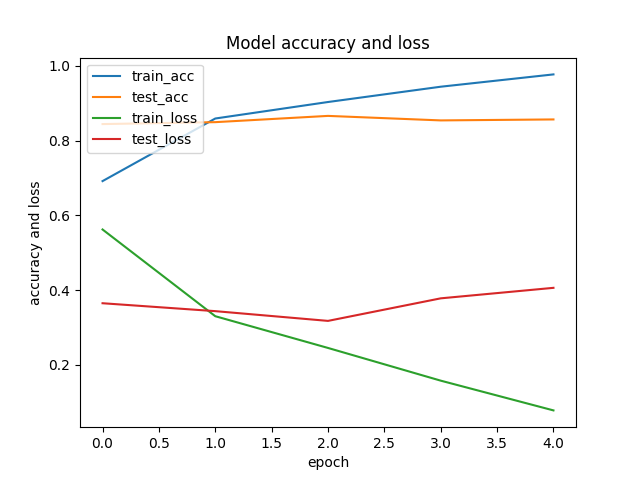
\includegraphics[width=\textwidth]{model0.png}
         \caption{Model 0.}
         \label{fig:model0}
\end{subfigure}
\hfill
\begin{subfigure}{0.32\textwidth}
         \centering
         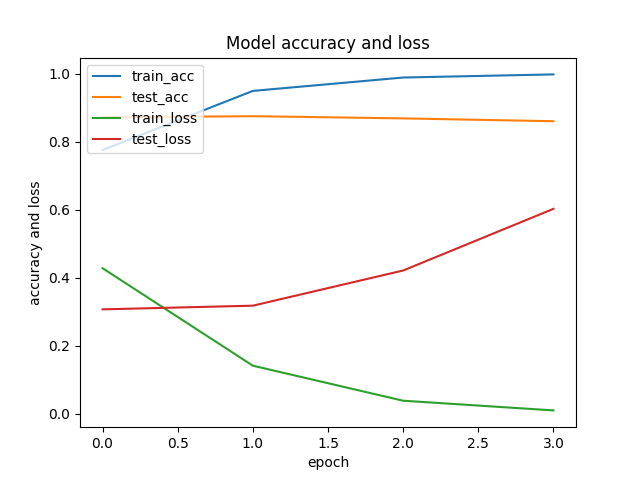
\includegraphics[width=\textwidth]{model1.png}
         \caption{Model 1.}
         \label{fig:model1}
\end{subfigure}
\hfill
\begin{subfigure}{0.32\textwidth}
         \centering
         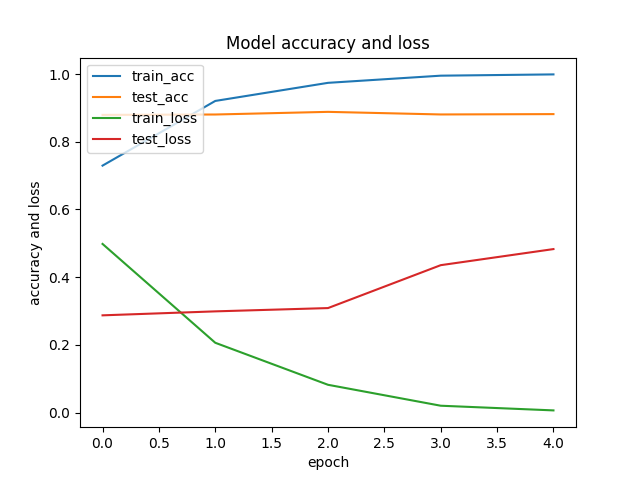
\includegraphics[width=\textwidth]{model2.png}
         \caption{Model 2.}
         \label{fig:model2}
\end{subfigure}
%
\begin{subfigure}{0.32\textwidth}
         \centering
         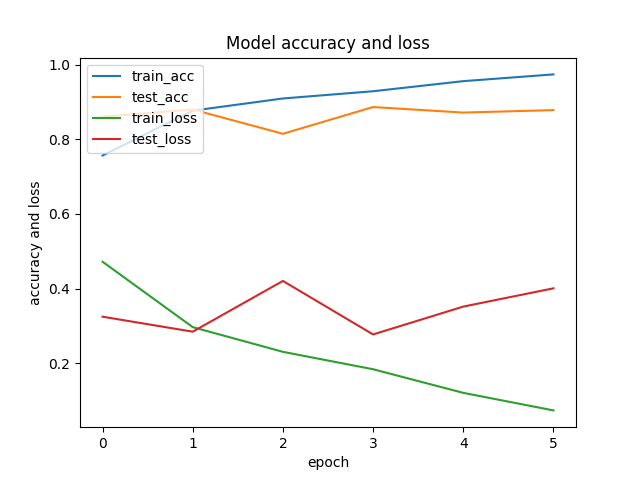
\includegraphics[width=\textwidth]{model3.png}
         \caption{Model 3.}
         \label{fig:model3}
\end{subfigure}
\hfill
\begin{subfigure}{0.32\textwidth}
         \centering
         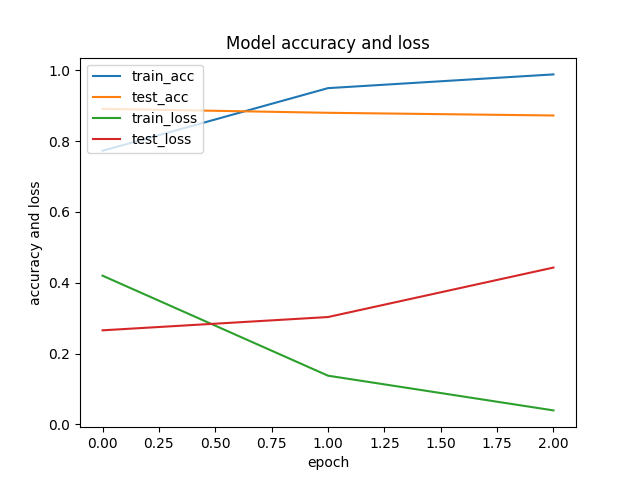
\includegraphics[width=\textwidth]{model4.png}
         \caption{Model 4.}
         \label{fig:model4}
\end{subfigure}
\hfill
\begin{subfigure}{0.32\textwidth}
         \centering
         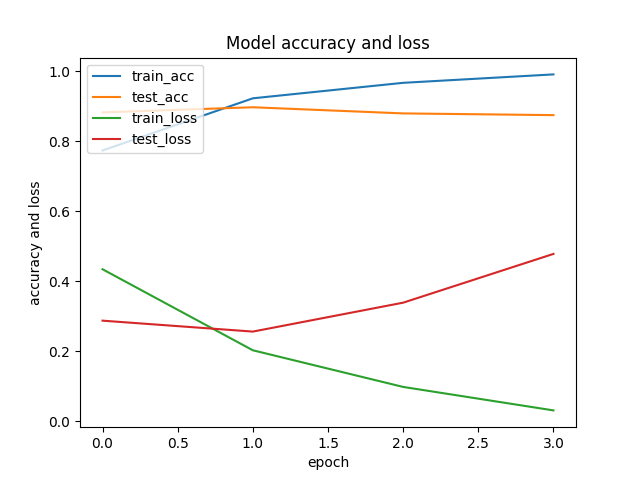
\includegraphics[width=\textwidth]{model5.png}
         \caption{Model 5 (\# filters = 96).}
         \label{fig:model5}
\end{subfigure}
\begin{subfigure}{0.32\textwidth}
         \centering
         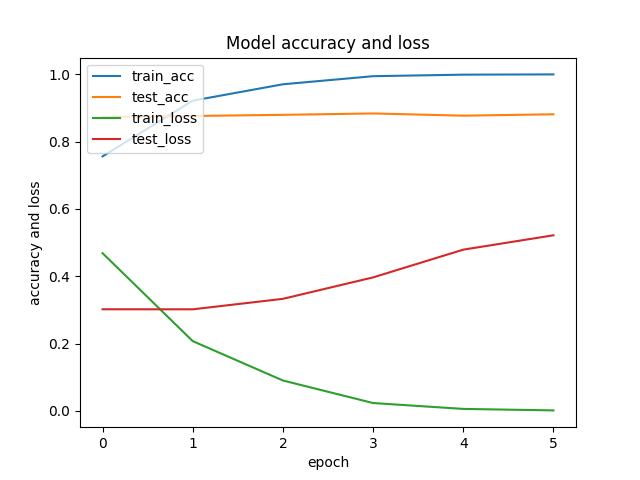
\includegraphics[width=\textwidth]{model6.png}
         \caption{Model 6.}
         \label{fig:model6}
\end{subfigure}
\hfill
\begin{subfigure}{0.32\textwidth}
         \centering
         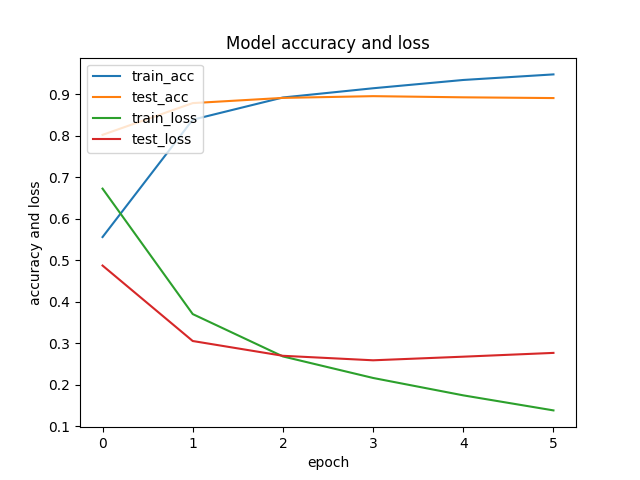
\includegraphics[width=\textwidth]{model7.png}
         \caption{Model 7.}
         \label{fig:model7}
\end{subfigure}
\hfill
\begin{subfigure}{0.32\textwidth}
         \centering
         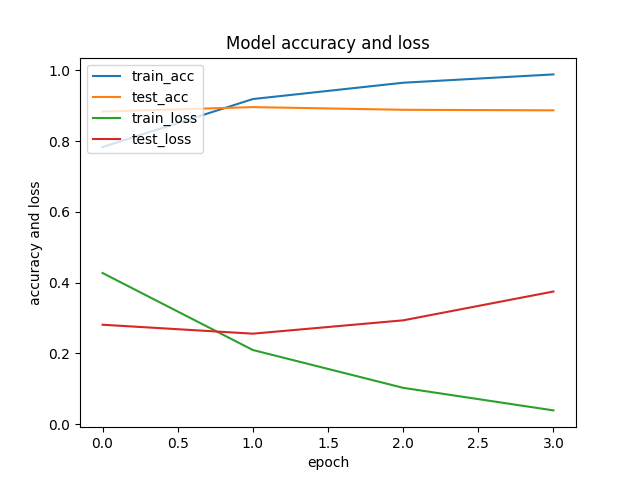
\includegraphics[width=\textwidth]{model8.png}
         \caption{Model 8 (\# filters = 48).}
         \label{fig:model8}
\end{subfigure}
\caption{Results of models on train and test dataset (X-axis: Epoch, Y-axis: accuracy and loss).}
\label{fig:accandlossmodel_overfitting}
\end{figure}
%====================

%====================
\begin{figure}[h!]
\centering
%
\begin{subfigure}{0.32\textwidth}
         \centering
         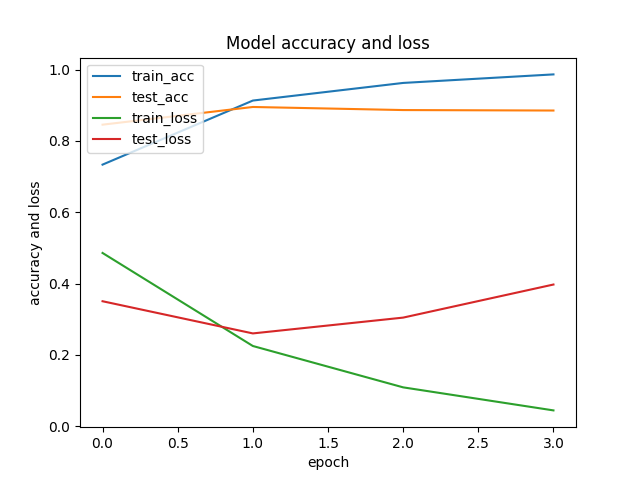
\includegraphics[width=\textwidth]{model9.png}
         \caption{Model 9 (\# filters = 24).}
         \label{fig:model9}
\end{subfigure}
\hfill
\begin{subfigure}{0.32\textwidth}
         \centering
         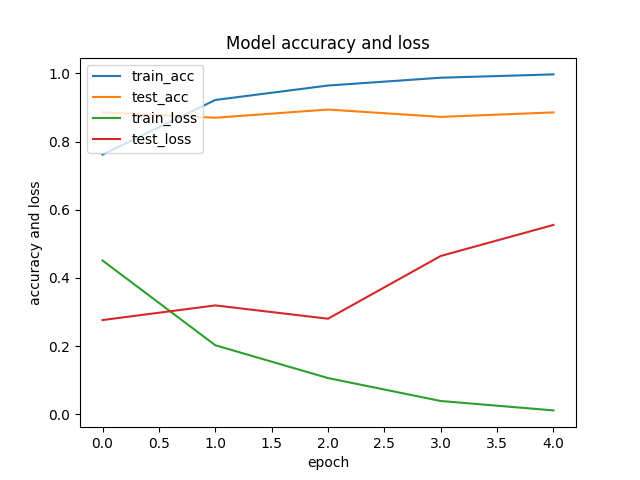
\includegraphics[width=\textwidth]{model10.png}
         \caption{Model 10 (\# units = 32).}
         \label{fig:model10}
\end{subfigure}
\hfill
\begin{subfigure}{0.32\textwidth}
         \centering
         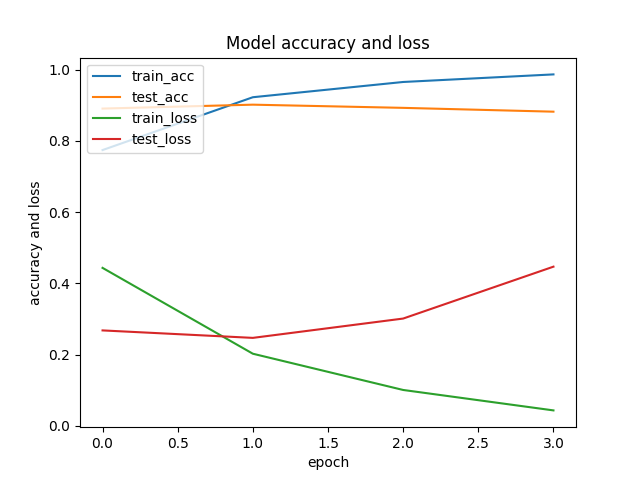
\includegraphics[width=\textwidth]{model11.png}
         \caption{Model 11 (\# units = 64).}
         \label{fig:model11}
\end{subfigure}
%
\begin{subfigure}{0.32\textwidth}
         \centering
         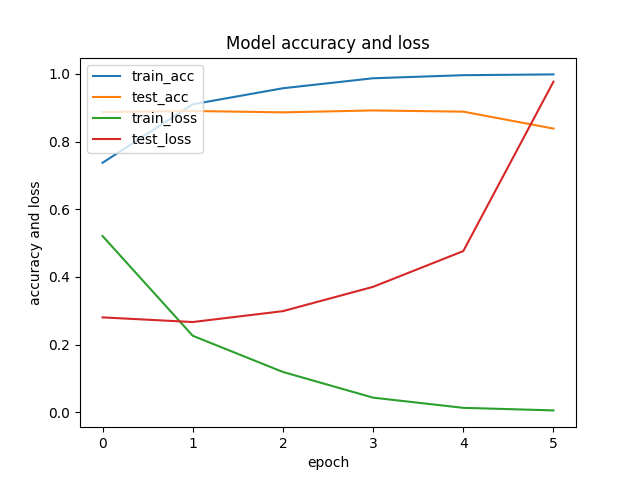
\includegraphics[width=\textwidth]{model12.png}
         \caption{Model 12 (\# units = 8).}
         \label{fig:model12}
\end{subfigure}
\hfill
\begin{subfigure}{0.32\textwidth}
         \centering
         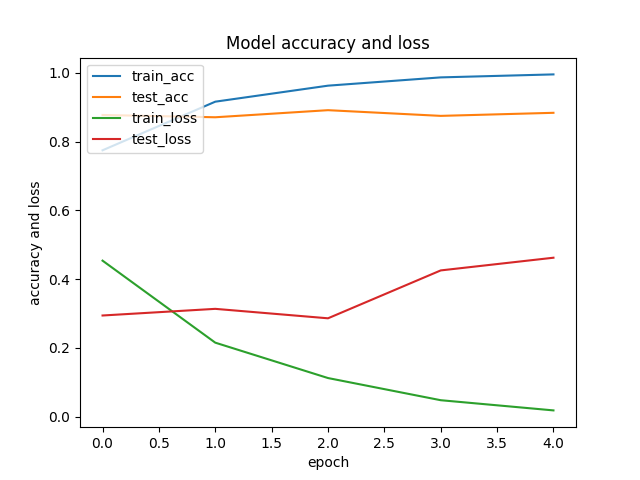
\includegraphics[width=\textwidth]{model13.png}
         \caption{Model 13.}
         \label{fig:model13}
\end{subfigure}
\hfill
\begin{subfigure}{0.32\textwidth}
         \centering
         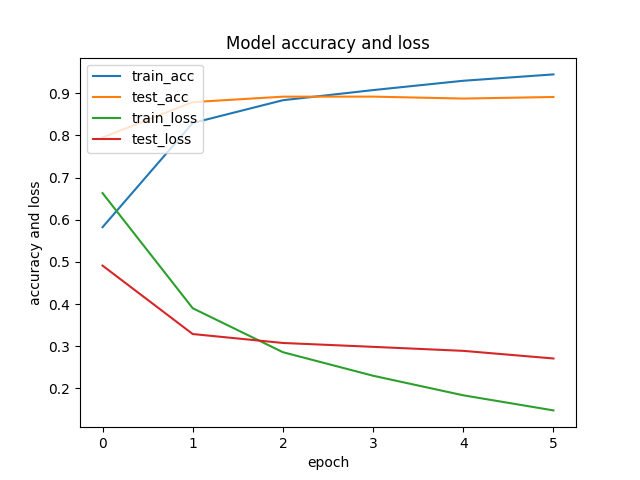
\includegraphics[width=\textwidth]{model14.png}
         \caption{Model 14.}
         \label{fig:model14}
\end{subfigure}
\begin{subfigure}{0.32\textwidth}
         \centering
         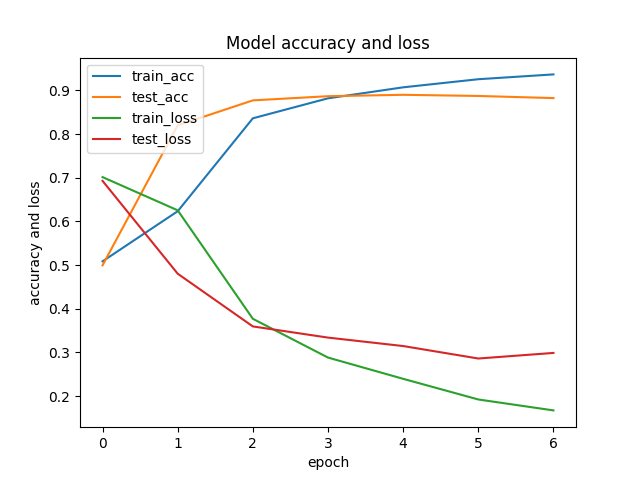
\includegraphics[width=\textwidth]{model15.png}
         \caption{Model 15.}
         \label{fig:model15}
\end{subfigure}
\hfill
\begin{subfigure}{0.32\textwidth}
         \centering
         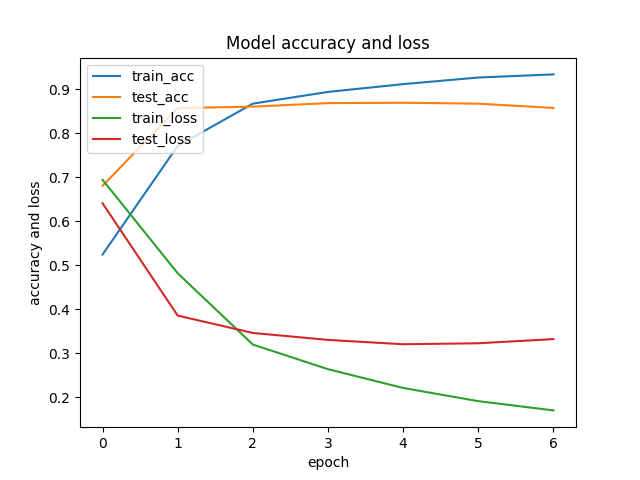
\includegraphics[width=\textwidth]{model16.png}
         \caption{Model 16.}
         \label{fig:model16}
\end{subfigure}
\hfill
\begin{subfigure}{0.32\textwidth}
         \centering
         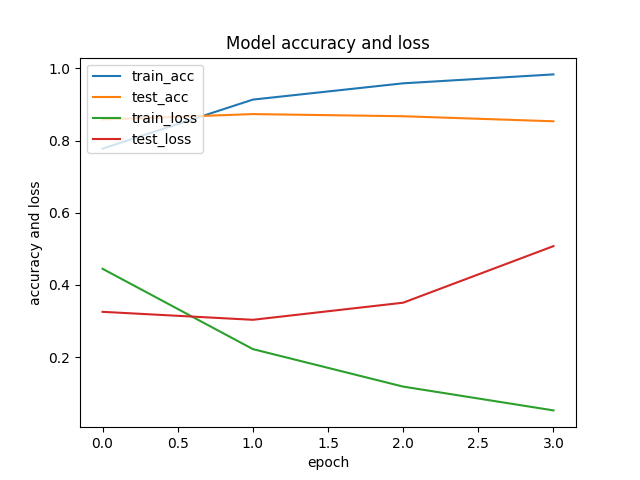
\includegraphics[width=\textwidth]{model17.png}
         \caption{Model 17.}
         \label{fig:model17}
\end{subfigure}
\caption{(Continued to Figure \ref{fig:accandlossmodel_overfitting}.) Results of models on train and test dataset (X-axis: Epoch, Y-axis: accuracy and loss).}
\label{fig:accandlossmodel_overfitting2}
\end{figure}
%====================
%overfitting
Figure \ref{fig:accandlossmodel_overfitting} and Figure \ref{fig:accandlossmodel_overfitting2} show 
the plots of accuracy and loss (y-axis) on every epoch (x-axis) for train and test data for deep learning models trained above.
%

Some of models seem to have the overfitting.
%
For example, in Model 12 in Figure \ref{fig:model12}, we can see that the test loss (red line) starts to increase as from epoch 4. The training loss (green line) continues to lower, which is normal as the model is trained to fit the train data as good as possible.
%
Just as with the test loss, the test accuracy peaks at the 4th epoch. After that, it goes down slightly. So to conclude, we can say that the model starts overfitting as from epoch 4.

%Effect of Reducing Network size and  (need to delete if only this is for the overfitting)
We applied \textbf{reducing the capacity of the network---i.e., lowering the number of convolutional layers, filters in convolutional layers, and hidden elements in the remaining layers (the units in Dense layers)---but it did not really help to avoid overfitting.}

%
It turned out that \textbf{adding Dropout layers help to prevent overfitting as in Figure \ref{fig:dropout_effect}.}
%
%
We can see that it takes more epochs to start overfitting than the no dropouts applied models.
%
For instance, in Figure \ref{fig:dropout1}, 
%the test loss starts increases later in the dropout applied model compared to the model with no dropouts ()
the model with no dropouts starts to increase the test loss from the epoch 1, while the dropout applied model starts at 5 epoch.
%
Moreover, the test loss increases much slower in the dropout applied model compared to the model with no dropouts (Figure \ref{fig:dropout2}). In short, the loss increases much slower afterwards.
%
This is because adding Dropout layers randomly remove certain features by setting them to zero.

%
As mentioned in Section \ref{Effect of Dropouts}, Dropouts lead the accuracy improvements only in the case of Figure \ref{fig:dropout4} (i.e., Model 6 when dropout=false to Model 7 when dropout=true) where the network size is small (i.e., number of filters are 24 and number of units are 32). 
%
It is apparent that the use of Dropouts continuously lowers the test loss while contributes to improve the test accuracy so that avoiding overfitting to find better solutions.

% the chance to find the global optimum so it sometimes should be used for proper training.
%even though Dropouts do not help improve accuracy, 
%Even though it does not help improve accuracy, it sometimes can be used for proper training. 

However, we decide that it is better to choose the model having the higher accuracy. 
\textbf{We do not sacrifice the accuracy but, to prevent overfitting, we used the EarlyStopping function to stop the training if the test accuracy dropped successively in two iterations (epochs)}.

%====================
\begin{figure}[h!]
\centering
\begin{subfigure}{0.35\textwidth}
         \centering
         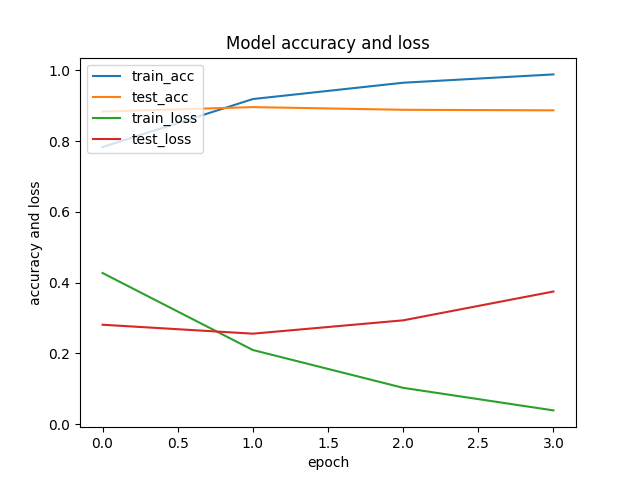
\includegraphics[width=\textwidth]{model8.png}
		 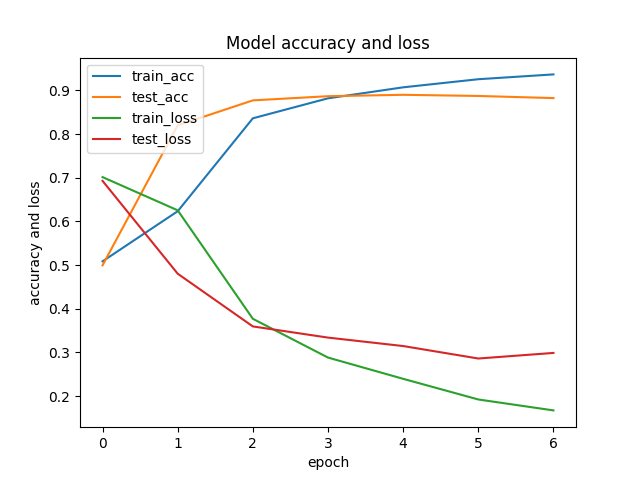
\includegraphics[width=\textwidth]{model15.png}
         \caption{Model 8 (Dropout=False) to Model 15 (Dropout = True).}
         \label{fig:dropout1}
\end{subfigure}
\hfill
\begin{subfigure}{0.35\textwidth}
         \centering
         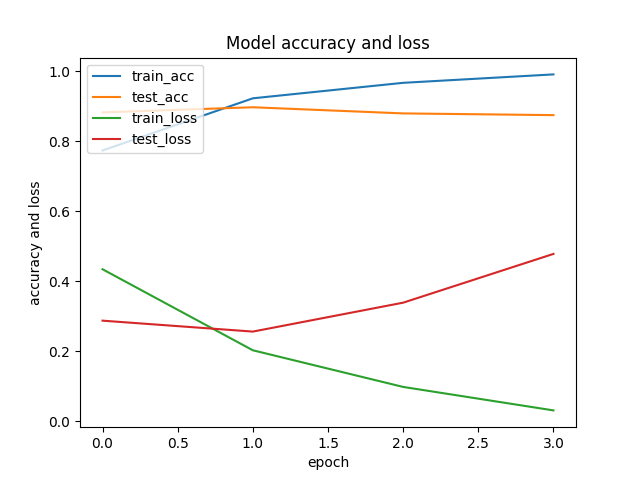
\includegraphics[width=\textwidth]{model5.png}
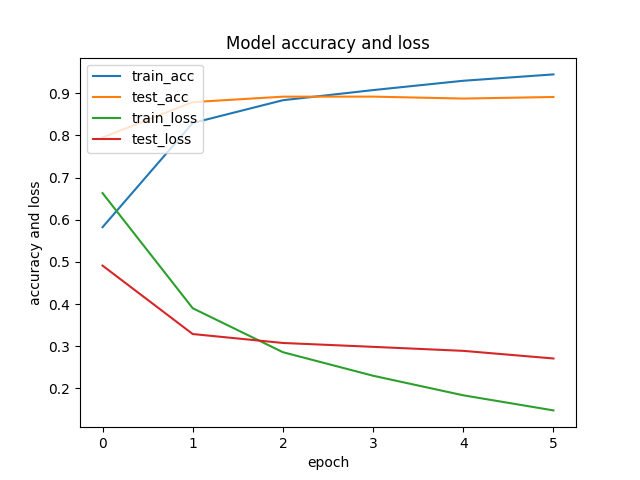
\includegraphics[width=\textwidth]{model14.png}
         \caption{Model 5 (Dropout = False) to Model 14 (Dropout = True).}
         \label{fig:dropout2}
\end{subfigure}
\hfill
\begin{subfigure}{0.35\textwidth}
         \centering
         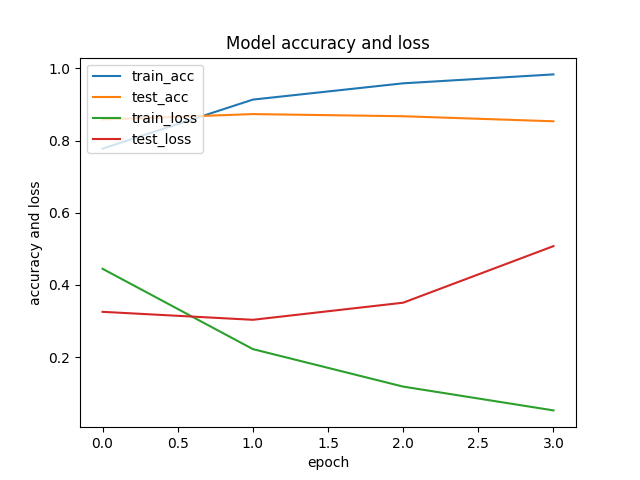
\includegraphics[width=\textwidth]{model17.png}
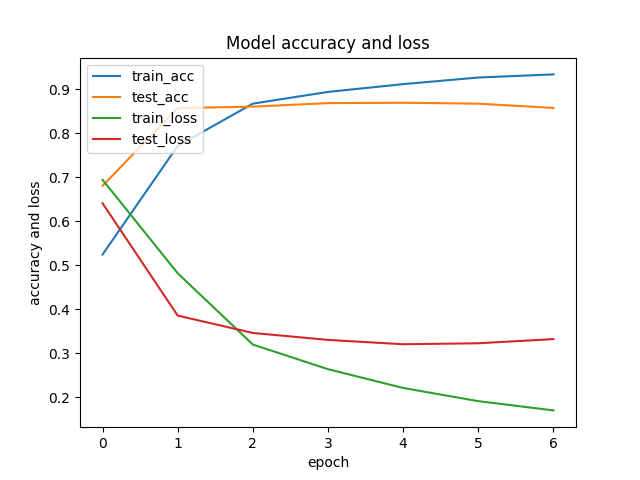
\includegraphics[width=\textwidth]{model16.png}

         \caption{Model 17 (Dropout = False) to Model 16 (Dropout = True).}
         \label{fig:dropout3}
\end{subfigure}
\hfill
\begin{subfigure}{0.35\textwidth}
         \centering
         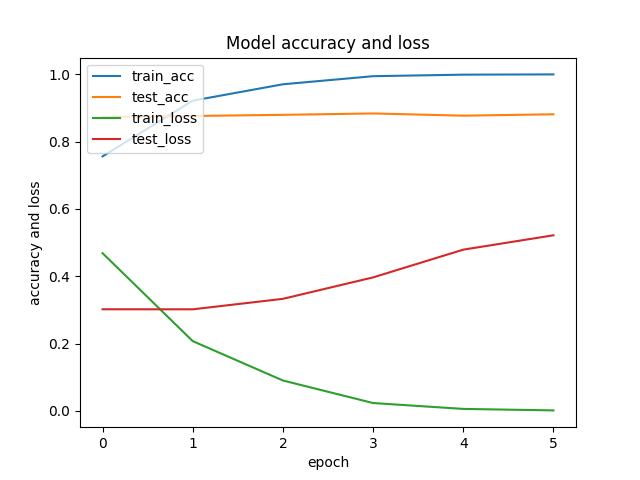
\includegraphics[width=\textwidth]{model6.png}
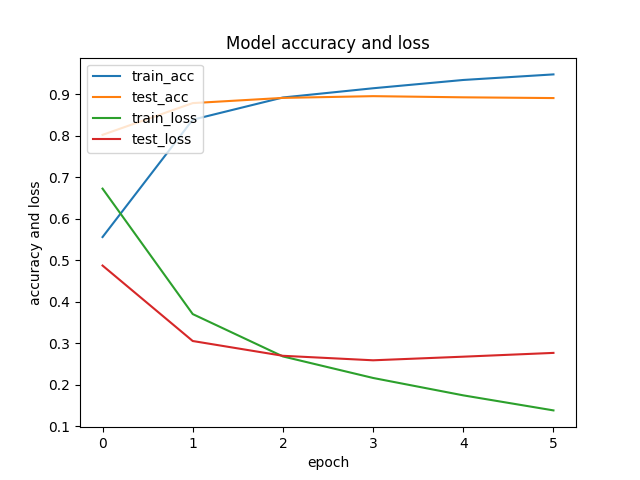
\includegraphics[width=\textwidth]{model7.png}
         \caption{Model 6 (Dropout = False) to Model 7 (Dropout = True).}
         \label{fig:dropout4}
\end{subfigure}
\caption{Dropout Effects on Overfitting.}
\label{fig:dropout_effect}
\end{figure}
%====================


\subsection{Limitation}

To improve the performance of accuracy, we can use the other techniques other than
reducing network size and adding dropouts 
to prevent overfitting in neural networks.
\begin{enumerate}
\setlength\itemsep{-1em}
%\item Reduce the capacity of the network.
%\item Add dropouts.
\item Get more training data.
\item Add weight regularization.
\item Data-augmentation.
\item Batch normalization.
\end{enumerate}

%
In the previous study \cite{Stanford_movie_review_paper}, the performance of machine learning models are in range of 67.42\% to 88.89\%. 
This model performed best in the cross validated Support Vector Machine (SVM) when concatenated with bag of words representation. 

%%%% important!!!
%
%In this project, the best accuracy of our deep learning models based on CNN is 90.14\%. 
In this project, the best model reaches 90.14\% classification accuracy on the test (validation) set at the first epoch. 
We could probably get to an even higher accuracy 
by 1) training longer with more overfitting preventing methods (such as dropout or regularization) or 
by 2) fine-tuning the Embedding layer.
%
However, this is the preliminary project for the classification of reviews using deep learning techniques.
We think this accuracy is enough to observe the advantages of using deep learning models on NLP problems. 
%
We will work further to improve the accuracy more of the deep learning models.

\section{Conclusion and Future Work}


%\paragraph*{Summary.}
In this project, we build deep learning models to classify the positive and negative movie reviews using the high-edge deep learning techniques. 

%
The process of building deep learning models is as follows.
We obtain the large data set of the movie reviews. 
We clean the documents of text reviews by removing punctuations, stopwords, stemming and removing non-frequent words to prevent a model from overfitting.
%
To build a deep learning Convolutional Neural Network (CNN) model, we basically use the sequential model of Keras. 
%
We used the three ways of setting the embedding layer: 1) using the pre-trained word embedding (GloVe embeddings), 2) training new embedding from scratch, and 3) both.
%
Then, a series of convolution 1D Neural Network and pooling layers are added according to typical CNN for text analysis. After flattening layer, fully connected Dense layers are added. To prevent overfitting, we add Dropouts to deactivate neurons randomly, which forces the network to learn a more balanced representation. We made different deep learning models by adjusting the parameters.

%results and findings
The best accuracy of our deep learning models based on CNN is 90.14\%.
The model produces the best accuracy
when documents are not cleaned,
the number of CNN is 3 (number of additional convolution layer is 2) with 96 filters,
pre-trained word embedding and training the Embedding layer are used, and
64 Dense layer is added without Dropouts.
%
%Dropout (avoid overfitting) vs. performance (accuracy)
Dropouts help to train data in better ways so 
that the loss of test starts to increase later or slower 
after using the Dropouts. 
%it not guarantee the best performance. 
But Dropouts do not guarantee the accuracy improvements.
Therefore, \textbf{the model with the highest accuracy is considered the best.}
%
In our project, to prevent overfitting, the training is stopped (EarlyStopping) 
when there is no more accuracy improvements, thus 
it is enough to use the models generated so far.
%The Dropouts help to avoid overfitting, but in our project, 

%%===============================
%summarize the brief findings
We summarize the findings as follows.
%word embedding
For the Word Embeddings, models that use the pre-trained word embedding and updating weights during training provide the best performance.
%CNN (# layers and #filters)
For the CNN and filters,
the model with 3 layers works better than the model with only one layer, but the difference is marginal. 
Likewise, the largest number of filters in CNN gives best performance, but it does not guarantee that the larger number of filters always produces the better performance.
%
Regarding to the units in Dense layers, the model with the 64 number of units in the Dense layer has the highest accuracy. Exception of that model, the larger number of units in the Dense layer has, the better performance.
%
For the use of the cleaned documents,
it seems that the cleaning degrades or does not improve the accuracy in our project.

%initial ideas on deep learning projects
%%===============================
For the future work, I will investigate another interesting projects using deep learning techniques. I have special interests in a photo caption generator. In this project, using the photo and text data for training, I aim to design and train a deep learning caption generation model, evaluate a train caption generation model, and use it to caption entirely new photographs.


For the final comment,
I give my special thanks to Tony Paek who has been my mentor for completing this project.

\newpage
\bibliography{scibib}
\bibliographystyle{Science}

%\bibliography{arhan}
%\bibliographystyle{IEEEtran.cls}

\end{document}


















